%%%% CAR-bench IJCAI Competition -- Track 2 Technical Report
\typeout{CAR-bench Track 2 Technical Report}

\documentclass{article}
\pdfpagewidth=8.5in
\pdfpageheight=11in

\usepackage{ijcai26}

\usepackage{times}
\usepackage{soul}
\usepackage{url}
\usepackage[hidelinks]{hyperref}
\usepackage[utf8]{inputenc}
\usepackage[small]{caption}
\usepackage{graphicx}
\usepackage{amsmath}
\usepackage{booktabs}
\usepackage{tikz}
\usetikzlibrary{shapes.geometric, arrows.meta, positioning, fit}

\urlstyle{same}

\pdfinfo{
/TemplateVersion (IJCAI.2026.0)
}

\title{A Budget-Gated Reliability Stack for Limit-Aware In-Car Agents:\\
CAR-bench Track 2 with an Open 120B Model}

\author{
Maximilian Stephan$^1$
\and
Simon Franken$^2$
\affiliations
$^1$University of Augsburg\\
$^2$Independent
\emails
maximilian.stephan@uni-a.de,
mail@simon-franken.de
}

\begin{document}

\maketitle

\begin{abstract}
We describe our Track~2 submission to the CAR-bench competition: an
agent built on the open-weight \texttt{gpt-oss-120b} model served by
Cerebras. Instead of scaling the model, we spend the track's inference
budget on \emph{reliability}. A three-stage pipeline --- constrained
generation with deterministic enforcement retries, a risk-gated LLM
verifier, and a bounded revision --- is hard-capped in code at the
track limit of five sequential LLM calls per baseline step, with the
cap enforced by a shared per-step budget rather than by convention.
Three deterministic guards add reliability at \emph{zero} additional
calls: phase separation (gather before acting), literal argument
traceability, and a capability-catalog diff that tells the agent which
ordinarily available tools are absent from the current session. On the
public test split our agent reaches $58.7\%$ Pass$^3$, up from $43.3\%$
for our prompt-only baseline, placing an open 120B model in the range
reported for substantially larger proprietary systems. We report
ablations, four techniques that \emph{failed}, and the measurement
noise floor that makes such comparisons fragile.
\end{abstract}

\section{Introduction}

CAR-bench evaluates whether an in-car assistant stays \emph{consistent}
and \emph{limit-aware} under real-world uncertainty
\cite{kirmayr2026carbench}. Its three task families probe distinct
failure modes: \textsc{base} measures ordinary task completion,
\textsc{hallucination} removes tools from the session and checks
whether the agent admits the limitation instead of fabricating a
result, and \textsc{disambiguation} checks whether ambiguity is
resolved from context or, when it cannot be, surfaced to the user.
Scoring is strict: a task counts only if tool use, final state,
intermediate state, and policy compliance are all correct, and we
report Pass$^3$ (all three trials of a task succeed), which punishes
non-determinism as hard as outright error.

Track~2 constrains inference rather than model choice: at most five
\emph{sequential} LLM calls per baseline step (parallel calls inside a
step are permitted) and at most 500k tokens per task on average. The
reference baseline uses one call per step. This framing invites a
specific question, which is the subject of this report: \emph{given a
mid-sized open model, what is the most score-efficient way to spend
four additional calls?}

Our answer is that most of the gain does not come from the extra calls
at all. The largest single improvement in our system is a
deterministic, zero-call prompt injection; the second largest is a
deterministic validator. The extra LLM calls are worth spending only
when they are \emph{gated} --- fired on a minority of steps that
heuristics flag as risky. We contribute: (i) a per-step call budget
that makes the track constraint a code invariant (Section~2);
(ii) a set of deterministic guards derived from CAR-bench's own error
taxonomy (Section~3); (iii) an evaluation showing $43.3\% \rightarrow
58.7\%$ Pass$^3$ with a per-technique breakdown (Section~4); and
(iv) an honest account of four techniques that did not survive
validation, plus the noise floor that nearly hid that fact
(Section~5).

\section{Architecture and Call-Budget Compliance}

\subsection{Unit of accounting}

We define one \emph{baseline LLM step} as one action generation: one
A2A round in which the agent receives a message and returns exactly one
action (tool calls or a user-facing response). This is the unit the
reference baseline serves with a single LLM call, and it corresponds
one-to-one to an invocation of \texttt{execute()} in our agent. The
budget is allocated and reset per invocation, so the constraint holds
per step by construction.

We stress this because the A2A token-reporting field
\texttt{turn\_metrics.num\_llm\_calls} aggregates over a whole
conversational \emph{turn} (several rounds of tool calling before the
agent finally speaks) and therefore legitimately exceeds five. Auditors
should read our per-step log line \texttt{sequential\_llm\_calls\_this\_step},
which is emitted once per baseline step.

\subsection{Pipeline}

Figure~\ref{fig:arch} shows the pipeline. Stage~\textcircled{1}
generates a next action under a JSON response schema that forces the
model to fill a \texttt{checks} object (\texttt{missing\_capability},
\texttt{unspecified\_value\_source}, \texttt{scope\_ok}) \emph{before}
naming an action, which acts as a short structured chain of thought.
The parsed action then passes three deterministic validators; a
violation raises a malformed-response error that triggers a retry
carrying a targeted correction, but never on the final permitted
attempt --- an inconsistent action is preferable to a turn error.

Stage~\textcircled{2} is an LLM verifier, deliberately narrow: it runs
only on state-changing actions, uses low reasoning effort and a 512
token cap, and returns \texttt{approve} or \texttt{revise} with
problems. A risk gate suppresses it entirely in the common,
uninteresting case --- a single state-changing call whose argument
values are all literally traceable to the conversation. Stage
\textcircled{3} is a single bounded revision seeded with the verifier's
problems. Neither stage can fail a turn: on any error the
stage~\textcircled{1} action stands.

\begin{figure}[t]
\centering
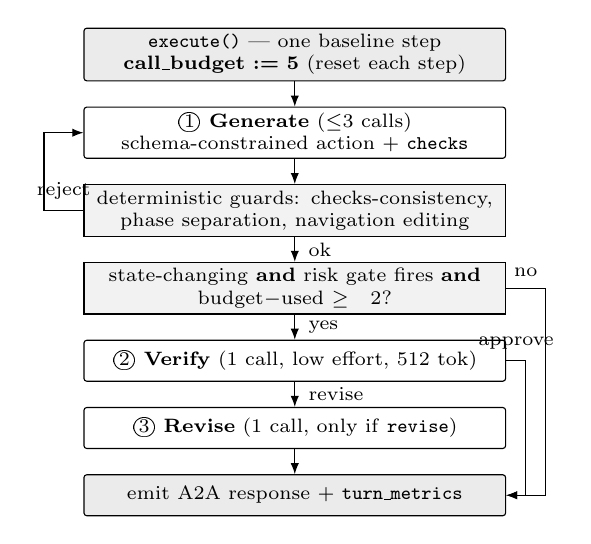
\begin{tikzpicture}[
  font=\scriptsize,
  node distance=3.2mm,
  box/.style={draw, rounded corners=1pt, align=center, inner sep=2.2pt,
              text width=52mm, minimum height=5.2mm},
  dec/.style={draw, align=center, inner sep=2.2pt, text width=52mm,
              minimum height=5.2mm, fill=black!5},
  arr/.style={-{Latex[length=1.4mm]}}
]
\node[box, fill=black!8] (ex) {\texttt{execute()} --- one baseline step\\
  \textbf{call\_budget := 5} (reset each step)};
\node[box, below=of ex] (s1) {\textcircled{1} \textbf{Generate}
  (\(\leq\)3 calls)\\
  schema-constrained action + \texttt{checks}};
\node[dec, below=of s1] (g) {deterministic guards: checks-consistency,\\
  phase separation, navigation editing};
\node[dec, below=of g] (rg) {state-changing \textbf{and} risk gate fires
  \textbf{and}\\ budget\(-\)used \(\geq 2\)?};
\node[box, below=of rg] (s2) {\textcircled{2} \textbf{Verify} (1 call,
  low effort, 512 tok)};
\node[box, below=of s2] (s3) {\textcircled{3} \textbf{Revise} (1 call,
  only if \texttt{revise})};
\node[box, below=of s3, fill=black!8] (out) {emit A2A response
  \(+\) \texttt{turn\_metrics}};

\draw[arr] (ex) -- (s1);
\draw[arr] (s1) -- (g);
\draw[arr] (g) -- node[right=0.5mm] {ok} (rg);
\draw[arr] (rg) -- node[right=0.5mm] {yes} (s2);
\draw[arr] (s2) -- node[right=0.5mm] {revise} (s3);
\draw[arr] (s3) -- (out);

\draw[arr] (g.west) -- ++(-5mm,0) node[midway, above=0.2mm] {reject}
  |- (s1.west);
\draw[arr] (rg.east) -- ++(5mm,0) node[midway, above=0.2mm] {no}
  |- (out.east);
\draw[arr] (s2.east) -- ++(2.5mm,0) node[midway, above=0.2mm]
  {approve} |- (out.east);
\end{tikzpicture}
\caption{One baseline LLM step. All stages draw from a single per-step
budget; the worst case is $3+1+1=5$ sequential calls, the common case is
$1$--$3$. No parallel calls are used.}
\label{fig:arch}
\end{figure}

\subsection{Why the bound holds}

Table~\ref{tab:budget} accounts for the worst case. The key mechanism
is that every stage receives the \emph{remaining} budget, not a private
allowance: stage~\textcircled{1} caps its attempts at
$\min(\text{retries}+1,\ \text{budget})$; the verifier runs only if at
least two calls remain (so that a revision it requests is always
affordable); the revision receives exactly what is left. An optional
completeness pass and a decline judge exist in the code but are
disabled in the submitted configuration; both share the same guard, so
the bound is independent of those toggles. Retries are counted as
calls, which is conservative --- a lenient reading would exclude them.

\begin{table}[t]
\centering
\begin{tabular}{@{}llcc@{}}
\toprule
& Stage & Max & Total \\
\midrule
\textcircled{1} & Generate ($1 + 2$ enforcement retries) & 3 & 3 \\
\textcircled{2} & Verify (gated: needs $\geq 2$ left)    & 1 & 4 \\
\textcircled{3} & Revise (gated: budget $-$ used)        & 1 & \textbf{5} \\
\bottomrule
\end{tabular}
\caption{Worst-case sequential calls per baseline step. Measured
average token use in the submitted configuration is ${\sim}92$k per
task against the 500k limit.}
\label{tab:budget}
\end{table}

\section{Reliability Techniques}
\label{sec:techniques}

\paragraph{Zero-call deterministic guards.}
Three validators inspect the parsed action and, on violation, force a
corrected regeneration within stage~\textcircled{1}.
\emph{Checks-consistency} rejects actions that contradict the model's
own self-report (e.g.\ declaring a missing capability and then changing
state anyway). \emph{Phase separation} implements the recommendation
from the CAR-bench analysis to separate information gathering from
execution: no state change without a prior read-only call, and no
clarifying question without a tool attempt since the last user message.
\emph{Navigation editing} forces the agent to observe navigation state
before replacing an active route --- exploiting a property of the
reward function, namely that intermediate-state credit is a
\emph{subset} check over state hashes, so additional read-only calls
are free while wrong state changes are not.

\paragraph{Argument-level anti-hallucination.}
Every argument of a state-changing call must appear literally in the
conversation (user utterance or tool result); values that are invented
or silently defaulted are rejected. A separate validator catches
template placeholders (\texttt{\{\{...\}\}}, \texttt{<...>},
\texttt{tbd}) that the model emits when chaining dependent calls. This
second validator alone moved \textsc{base} from $62\%$ to $66$--$72\%$,
mostly on multi-step route lookups.

\paragraph{Capability-catalog notice.}
The agent ships a static catalog of the tools and parameters that are
ordinarily present in this domain, compiled from the public training
split. At prompt-construction time it diffs the catalog against the
tools the evaluator actually supplied and, if anything is missing,
injects a notice naming the gap and instructing the agent to say
plainly that it cannot do that part --- and not to ask the user to
supply it, claim success, or fake a workaround. This is a static prompt
prior, not runtime introspection: the diff consumes only
evaluator-provided tool definitions, and the resulting behaviour stays
fully visible to the hallucination metric. It is our single largest
win (\textsc{hallucination} $42\% \rightarrow 52$--$54\%$, twice
confirmed) and fired zero times across all 75 \textsc{base} and
\textsc{disambiguation} tasks, i.e.\ it is inert where it should be.
Two smaller injections follow the same pattern: a toll-disclosure
reminder when a retrieved route sets \texttt{includes\_toll}, and a
notice not to re-ask for information the user has just declined to
provide.

\paragraph{Gated verification.}
Over a full run the verifier issued 86 reviews and requested revision
in $21\%$ of them; inspection of a sample showed substantive catches
(a policy violation, invented values, unrequested extra actions) rather
than stylistic nagging. Gating matters: the full stack costs only
$+13\%$ LLM time versus the single-call baseline, because most steps
never reach stage~\textcircled{2}.

\section{Results}

\begin{table}[t]
\centering
\begin{tabular}{@{}lcccc@{}}
\toprule
Configuration & Base & Hall. & Dis. & \textbf{Pass$^3$} \\
\midrule
Prompt-only baseline      & 60 & 42 & 28 & 43.3 \\
$+$ guards, gated verifier & 64 & 42 & 48 & 51.3 \\
$+$ catalog notice        & 62 & 54 & 40 & 52.0 \\
$+$ placeholder, toll     & 66 & 58 & 52 & \textbf{58.7} \\
\midrule
\emph{confirmation run}   & 72 & 58 & 40 & 56.7 \\
\bottomrule
\end{tabular}
\caption{Pass$^3$ (\%) on the public test split, 125 tasks
$\times$ 3 trials, temperature $0$. Rows are cumulative
configurations, each measured in a separate full run.}
\label{tab:results}
\end{table}

Table~\ref{tab:results} reports full runs on the public test split
(125 tasks, three trials, temperature $0$; Pass$^3$ is averaged over
the three task families). Every row is a separate full evaluation.
Reaching the final configuration took 16 such runs --- roughly an hour
of wall-clock time each --- alongside 30 shorter runs on task subsets,
over eight days. We report full-run numbers exclusively: as
Section~\ref{sec:noise} shows, the short runs we used for iteration
were systematically misleading, and several configurations that looked
best on a subset lost on the full split. The stack raises Pass$^3$
from $43.3\%$ to $58.7\%$, with the best configuration confirmed twice
in the $56$--$59\%$ range. For context, the published CAR-bench
leaderboard places the same open model at $28\%$ and reports $41\%$ for
\texttt{gemini-2.5-flash-thinking} and $54\%$ for
\texttt{GPT-5-thinking}; our figures are not directly comparable
(different split conditions and user-simulator routing), but the gap
between $28\%$ and $58.7\%$ for one and the same open model is the
result we consider meaningful.

The per-family pattern is informative. \textsc{Disambiguation}
responds to structural interventions (phase separation fired 170 times
in one run and lifted the family $28 \rightarrow 48$), whereas
\textsc{hallucination} responds almost exclusively to the catalog
notice. The two families also interfere: a preference-consultation
rule that solved several \textsc{disambiguation} tasks eroded
\textsc{hallucination} consistency, an instance of the
completion-versus-compliance tension the CAR-bench authors describe.

\section{Negative Results and Measurement Noise}
\label{sec:noise}

We report four techniques that looked promising and did not survive.
(i)~A \emph{workflow memory} mined from the training split (canonical
tool prerequisites, 312 tokens) scored $73\%$ on a focused slice but
$48.0\%$ on a full run versus $51.3\%$; the prime suspect is a
``let the user choose'' phrasing that induced asking in tasks requiring
internal resolution. (ii)~A \emph{response scaffold} forcing an
explicit cannot-statement plus fallback offer produced the first-ever
full flips on our stubborn missing-response class in focused runs, yet
that class flipped back at the run level despite 88 activations; after
seven attempts we closed it as a model-capability limit.
(iii)~A \emph{completeness verifier} raised Pass@3 to $80\%$ while
Pass$^3$ \emph{fell} from $52.0\%$ to $44.7\%$: 109 self-second-guessing
revisions turned thirteen stable tasks flaky --- a reminder that under
Pass$^3$, variance is a first-class cost. (iv)~An \emph{enrichment
rule} for user preferences gained one task and broke our most stable
marker task.

These conclusions are only possible because we first measured the noise
floor. At temperature $0$ the three trials of a run are near-clones, so
borderline tasks flip at the \emph{run} level rather than the trial
level; an identical configuration measured twice on a 15-task slice
produced $66\%$ and $46\%$. We therefore accept a change only when it
is deterministic (a $0/x \rightarrow x/x$ flip) or reproduces across at
least two independent full runs, and we treat $\pm 8$pp on
\textsc{disambiguation} as noise. A second, non-obvious confound: the
evaluator's user simulator is itself an LLM, and provider congestion
truncated its JSON badly enough to produce a $18.7\%$ run that had
nothing to do with agent quality. Run-level evaluator error counts
correlate with score and must be checked before any comparison.

\paragraph{Where the remaining errors live.}
To decide when to stop, we classified the deterministically failing
tasks of our best run by root cause. Only about four of thirty were
cleanly addressable by harness work. The remainder split into
route or destination selection (5 tasks, a reasoning failure),
under-acting and omitted actions (4, semantics), final state diverging
from ground truth (4, reasoning), navigation state that is simply not
observable unless the agent chooses to look (5), and content or
formatting requirements such as toll disclosure and 24-hour times.
This distribution is why we stopped adding mechanisms: the harness can
enforce structure and surface facts, but it cannot supply reasoning the
underlying model does not have. It also explains the asymmetry in
Table~\ref{tab:results} --- interventions that convert an
\emph{observability} gap into an explicit prompt fact (the catalog
notice, the navigation-state guard) pay off immediately, whereas the
reasoning-bound classes barely move.

\section{Compliance and Reproducibility}

\begin{table}[t]
\centering\small
\begin{tabular}{@{}lp{56mm}@{}}
\toprule
Enabled & \texttt{MAX\_CALLS\_PER\_STEP}=5, \texttt{VERIFIER},
  \texttt{VERIFIER\_GATE}, \texttt{ENFORCE\_CHECKS},
  \texttt{PHASE\_SEPARATION}, \texttt{NAV\_EDITING},
  \texttt{CATALOG\_NOTICE}, \texttt{TOLL\_NOTICE}\\
\midrule
Disabled & \texttt{COMPLETENESS}, \texttt{WORKFLOWS},
  \texttt{RESPONSE\_SCAFFOLD}, \texttt{DECLINE\_JUDGE}\\
\midrule
Sampling & temperature $0$, $2048$ completion tokens,
  $2$ enforcement retries, verifier effort \texttt{low}\\
\bottomrule
\end{tabular}
\caption{Submitted configuration. Every entry is an environment
variable with the stated value as its default in the submitted
\texttt{scenario.toml}, so the configuration is reproduced even when
nothing is injected but the API key.}
\label{tab:config}
\end{table}

The submitted agent uses Cerebras-hosted \texttt{gpt-oss-120b} through
the Cerebras SDK, with all model names, routes, API bases, service
tiers, reasoning-effort selectors and sampling parameters exposed as
environment variables in the submitted \texttt{scenario.toml}; the
organizers need only supply the API key. The agent uses exclusively
evaluator-provided inputs --- system and policy text, transcript, tool
definitions, tool results --- plus the static public-domain catalog
described in Section~3. It does not execute CAR-bench tools, read
hidden task state or answer keys, or add private tools to the decision
loop, and it reports \texttt{prompt\_tokens}, \texttt{completion\_tokens}
and \texttt{thinking\_tokens} on final responses. The image is public
and digest-pinned; it was validated end-to-end against the official
evaluator image via the repository's GHCR validation path.
Table~\ref{tab:config} lists the exact submitted configuration.

Two caveats belong on the record. First, the capability catalog of
Section~\ref{sec:techniques} is prior knowledge: it is compiled offline
from the \emph{public} training split and shipped as a static file. It
contains no task, answer or hidden-state information and is never
updated at run time, but it does encode the expectation that a session
normally offers a particular set of tools. Second, our development
numbers were produced with the evaluator's user simulator and policy
judge routed through a third-party provider rather than the organizers'
configuration; scores are therefore internally comparable but not
directly comparable to published leaderboard figures.

\section{Limitations and Future Work}

Our development loop iterated on a fixed public split, and we measured
the resulting selection bias directly: at an early stage of
development, tasks we had been tuning against scored roughly $70\%$
while unseen tasks of the same run scored about $43\%$, with unseen
\textsc{disambiguation} as low as $13\%$. We reacted by validating only
on full runs and by preferring mechanisms that are deterministic and
domain-general --- a guard that enforces ``observe before replacing an
active route'' encodes a domain rule, not a task --- but some
adaptation to the public split certainly remains, and the hidden-set
result should be expected to fall below our development figure.

Three directions remain open. First, the verifier currently checks
several aspects in one pass; splitting it into narrow single-aspect
reviewers is affordable within the call budget and may raise its
$21\%$ revision rate to a more useful precision. Second, best-of-$N$
sampling is attractive under Pass$^3$ but interacts badly with
provider rate windows, so it needs a scheduling story before it can be
evaluated fairly. Third, our workflow-memory experiment failed for what
looks like a single phrasing choice rather than a conceptual reason;
mined canonical tool orderings deserve a second attempt with the
offending route-selection line removed and \textsc{disambiguation}
validated separately.

\section{Conclusion}

Spending a fixed inference budget on \emph{gated} verification and
\emph{deterministic} guards, rather than on uniformly deeper reasoning,
lifted an open 120B model by more than 15 points of Pass$^3$ on
CAR-bench. The most transferable lesson is that the cheapest
interventions dominated: a static capability diff and an argument
validator, both costing no additional LLM calls, account for the
majority of the gain, while the one technique that added
\emph{ungated} model calls actively hurt by injecting variance into a
metric that punishes it. Limit-awareness, in our experience, is less a
reasoning problem than a plumbing problem.

\bibliographystyle{named}
\begin{thebibliography}{1}

\bibitem{kirmayr2026carbench}
Johannes Kirmayr, Lukas Stappen, and Elisabeth Andr\'e.
\newblock {CAR-bench}: Evaluating the consistency and limit-awareness of
  {LLM} agents under real-world uncertainty.
\newblock arXiv:2601.22027, 2026.

\end{thebibliography}

\end{document}
